\documentclass[10pt,a4paper]{article}

% ─── Packages ─────────────────────────────────────────
\usepackage{fontspec}
\setmainfont{Times New Roman}

\usepackage[top=1.1cm,bottom=1.1cm,left=1.55cm,right=1.55cm]{geometry}
\usepackage{titlesec}
\usepackage{enumitem}
\usepackage{hyperref}
\usepackage{xcolor}
\usepackage{tabularx}
\usepackage{graphicx}
\usepackage{parskip}

% ─── Colors ───────────────────────────────────────────
\definecolor{primary}{RGB}{30,40,90}
\definecolor{namecolor}{RGB}{0,120,180}
\definecolor{accent}{RGB}{50,90,150}
\definecolor{rulecol}{RGB}{200,205,220}
\definecolor{gray}{RGB}{90,90,90}

\hypersetup{
    colorlinks=true,
    urlcolor=accent
}

\pagestyle{empty}
\setlength{\parskip}{0pt}

% ─── Section ──────────────────────────────────────────
\titleformat{\section}
    {\normalsize\bfseries\color{primary}}
    {}
    {0em}
    {}
    [\vspace{1pt}\textcolor{rulecol}{\titlerule[0.6pt]}\vspace{1pt}]

\titlespacing{\section}{0pt}{5pt}{2pt}

% ─── Entry ────────────────────────────────────────────
\newcommand{\entry}[3]{%
    \noindent
    \begin{tabularx}{\linewidth}{X r}
        \textbf{\color{primary}#1} &
        {\scriptsize\color{gray}#2}
    \end{tabularx}\\[-2pt]
    {\scriptsize\textit{\color{gray}#3}}
    \vspace{1pt}
}

% ─── Compact list ─────────────────────────────────────
\newenvironment{cvitems}{
    \begin{itemize}[
        leftmargin=1.15em,
        topsep=0pt,
        itemsep=0.5pt,
        parsep=0pt,
        partopsep=0pt
    ]
}{
    \end{itemize}
}

% ═════════════════════════════════════════════════════
\begin{document}

% ─── HEADER ───────────────────────────────────────────
\noindent
\begin{tabularx}{\linewidth}{@{}X r@{}}

\begin{minipage}[c]{\linewidth}

    {\LARGE\bfseries\color{namecolor} Ho Huynh Nhu}\\[2pt]

    {\large\bfseries\color{primary}
    Quality Supervision Officer}\\[3pt]

    {\scriptsize\color{gray}
    20/10/2003
    \enspace\textcolor{rulecol}{|}
    \enspace (+84) 367 503 477
    \enspace\textcolor{rulecol}{|}
    \enspace
    \href{mailto:hhnhu2003@gmail.com}{hhnhu2003@gmail.com}
    \enspace\textcolor{rulecol}{|}
    \enspace Ho Chi Minh City}\\[2pt]

    {\scriptsize
    \href{https://github.com/hohuynhnhu}
    {github.com/hohuynhnhu}
    \enspace\textcolor{rulecol}{|}
    \enspace
    \href{https://www.facebook.com/huynhnhu.ho.961}
    {facebook.com/huynhnhu.ho.961}
    }

\end{minipage}

&

\begin{minipage}[c]{2.2cm}
    \raggedleft
    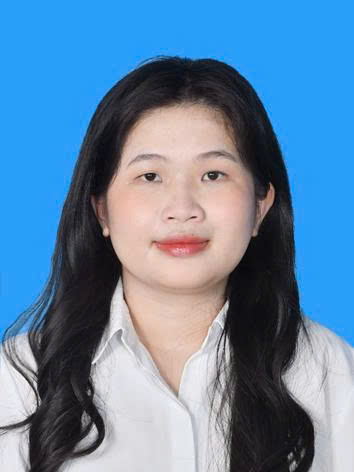
\includegraphics[
        width=2.2cm,
        height=2.7cm,
        keepaspectratio
    ]{assets/avt.jpg}
\end{minipage}

\end{tabularx}

\vspace{3pt}
\textcolor{rulecol}{\rule{\linewidth}{0.6pt}}

% ─── CAREER OBJECTIVE ─────────────────────────────────
\section*{Career Objective}

{\small
Final-year Information Technology student seeking a Quality Supervision
position. Experienced in building AI-based vehicle recognition and monitoring
systems with IoT sensors, tracking data in real time, detecting anomalies,
and preparing reports. Meticulous, responsible, and disciplined in following
assignments, with a strong wish to apply technology to improve service
quality and compliance with company procedures.
}

% ─── EDUCATION ────────────────────────────────────────
\section*{Education}

\entry
{University of Transport Ho Chi Minh City (UTH)}
{10/2022 -- 10/2026}
{Bachelor of Information Technology -- Completed coursework}

{\small
\begin{cvitems}
    \item GPA: 3.4 / 4.0
    \item \textbf{Excellent Scholarship} -- Semester 1, 2025
    \item \textbf{Second Prize -- AI Track},
    UTH Student Scientific Research Conference 2025
\end{cvitems}
}

% ─── FEATURED PROJECTS ────────────────────────────────
\section*{Featured Projects}

\entry
{VehicleScan -- Smart Vehicle Recognition \& Monitoring System}
{Python \textbar{} YOLO \textbar{} CNN \textbar{} Siamese Network \textbar{} ESP32 \textbar{} Kafka \textbar{} PostgreSQL \textbar{} Firebase}
{08/2025 -- 01/2026}

{\small
\begin{cvitems}

    \item Built an AI-based vehicle recognition system combined with IoT sensors (ESP32) to manage and monitor parking in real time.

    \item Prepared and labeled image datasets for vehicle detection, classification, and recognition tasks.

    \item Trained and evaluated YOLO, CNN, and Siamese Network models to detect, recognize, and identify vehicles.

    \item Applied image preprocessing and feature extraction to improve recognition accuracy under real-world image conditions.

    \item Designed data processing workflows for vehicle and IoT sensor data with Kafka, storing and managing data in PostgreSQL and Firebase.

    \item Integrated data from AI models, sensors, and the application into one unified system to track operating status and support timely decisions.

    \item Achieved \textbf{Second Prize -- AI Track} at the UTH Student Scientific Research Conference 2025.

    \item GitHub: \href{https://github.com/LeKhang-cn22h/VehicleScanner}{VehicleScanner}

\end{cvitems}
}

\vspace{3pt}

\entry
{Fall Detection -- Video-Based Monitoring \& Fall Detection System}
{Python \textbar{} PyTorch \textbar{} YOLOv8 Pose \textbar{} MediaPipe \textbar{} Transformer}
{04/2026 -- 06/2026}

{\small
\begin{cvitems}

    \item Extracted human pose features from video using MediaPipe and YOLOv8 Pose to detect fall incidents.

    \item Trained a Transformer Encoder model, achieving 97.8\% mean accuracy with 5-fold cross-validation and testing on unseen data.

\end{cvitems}
}

% ─── TECHNICAL SKILLS ─────────────────────────────────
\section*{Technical Skills}

{\small
\begin{tabularx}{\linewidth}{@{}lX@{}}

\textbf{Camera / AI Monitoring}
&
Object detection and recognition from images/video (YOLO, CNN, Siamese Network, MediaPipe),
Image Preprocessing, Model Evaluation
\\[1pt]

\textbf{IoT \& Real-time Monitoring}
&
ESP32, Kafka, RabbitMQ, Firebase, Real-time Data Tracking,
Anomaly Detection
\\[1pt]

\textbf{Data \& Reporting}
&
Python, SQL, PostgreSQL, Power BI, Excel, Operational Reporting, KPI Analysis
\\[1pt]

\textbf{Automation}
&
ETL/ELT, dbt, Apache Airflow, Docker

\end{tabularx}
}

% ─── WORK EXPERIENCE ──────────────────────────────────
\section*{Work Experience}

\entry
{Gotik Consulting -- Data Engineer}
{Python \textbar{} dbt \textbar{} PostgreSQL \textbar{} Airflow \textbar{} Power BI}
{03/2026 -- 05/2026}

{\small
\begin{cvitems}

    \item Processed, checked, and standardized Odoo business data to detect inconsistencies and prepare accurate datasets for reporting.

    \item Monitored hourly ETL workflows on Airflow, detecting and resolving failures promptly to keep the system stable.

    \item Built Power BI dashboards to monitor operational metrics and prepared regular reports.

\end{cvitems}
}

% ─── ADDITIONAL INFORMATION ───────────────────────────
\section*{Additional Information}

{\small
\begin{tabularx}{\linewidth}{@{}lX@{}}

\textbf{Soft Skills}
&
Following assignments \textbar{} Meticulous and responsible \textbar{}
Teamwork \textbar{} Timely reporting \textbar{} Problem-solving
\\[2pt]

\textbf{English}
&
Technical document reading and basic professional communication
\\[2pt]

\textbf{Availability}
&
Available for full-time opportunities.

\end{tabularx}
}

\end{document}